\documentclass[a4paper]{report}
\usepackage[spanish]{babel}
\selectlanguage{spanish}
\usepackage[utf8]{inputenc}
\usepackage[T1]{fontenc}
\usepackage{pdfpages}
\usepackage[a4paper,top=2cm,bottom=2cm,left=2cm,right=2cm]{geometry}
\usepackage{amsmath, amsthm, amsfonts}
\usepackage{graphicx}
\usepackage{minitoc}
\usepackage{color}
\usepackage{listings}
\usepackage{hyperref}
\usepackage{multicol}
\usepackage{float}
\usepackage{array}
\usepackage[none]{hyphenat}
\usepackage{appendix}
\usepackage[pdf]{graphviz}

\hypersetup{
    colorlinks=true, % make the links colored
    linkcolor=black, % color TOC links in blue
    urlcolor=red, % color URLs in red
    linktoc=all % 'all' will create links for everything in the TOC
}

\lstset{
basicstyle=\ttfamily,
captionpos=b,
frame=single,
texcl=true
}

\def\blankpage{%
      \clearpage%
      \thispagestyle{empty}%
      \addtocounter{page}{0}%
      \null%
      \clearpage}
    
\title{Desarrollo de la Lógica Proposicional y de Primer Orden bajo el paradigma funcional y la orientación Web.}
\author{Víctor Ramos González\\\\
   Tutor: Fernando Sancho Caparrini\\
   \textit{Ciencias de la Computación e Inteligencia Artificial}\\
   E.T.S. Ingeniería Informática\\
   Universidad de Sevilla\\
  \vspace{8cm}
  \date{Curso 2019/20}
}

\newcolumntype{P}[1]{>{\centering\arraybackslash}p{#1}}



\setlength{\parskip}{1em} 
 
\sloppy
\begin{document}

\renewcommand{\tablename}{Tabla}
\renewcommand{\appendixname}{Anexo}
\renewcommand{\appendixtocname}{Anexos}
\renewcommand{\appendixpagename}{Anexos}

\dominitoc

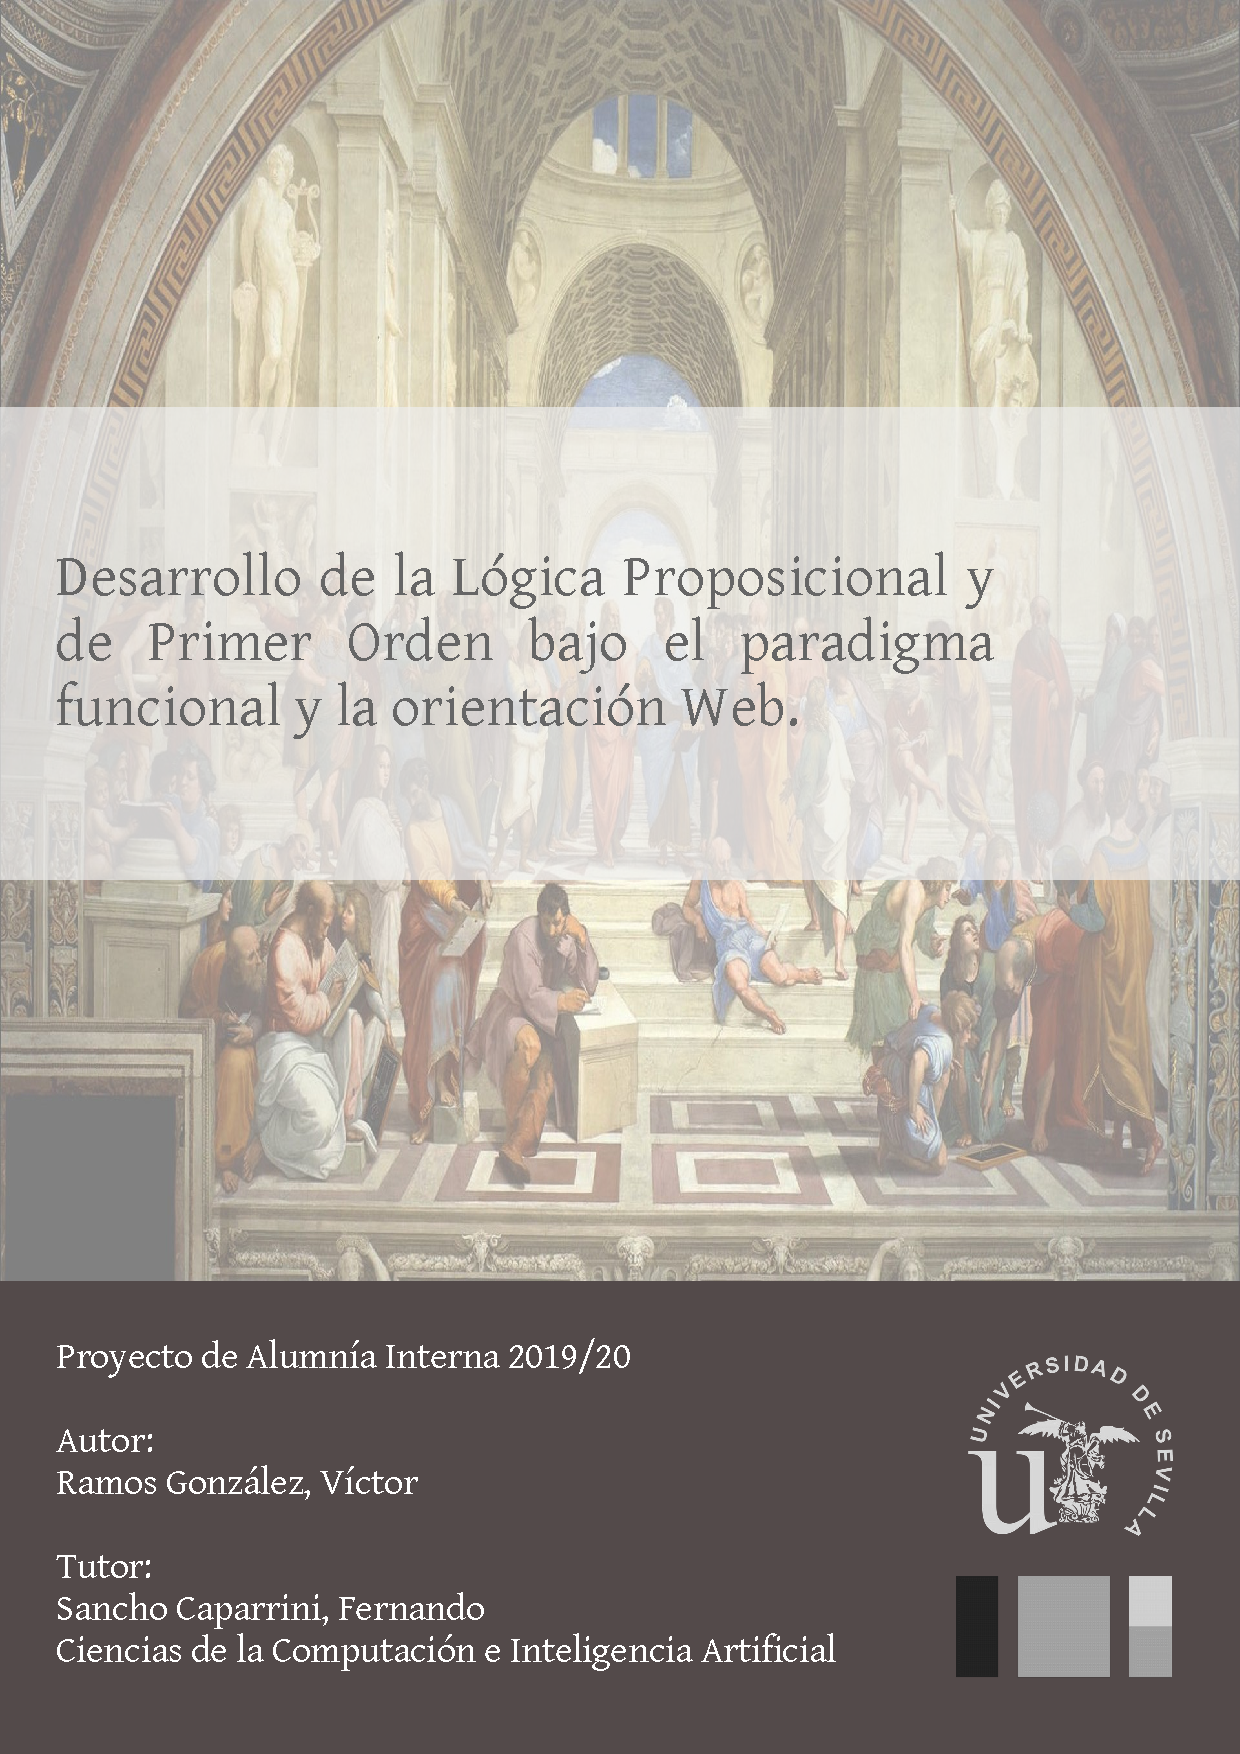
\includepdf[pages={1}]{archivos/titlepage.pdf}


\blankpage

\maketitle

\begin{abstract}

El proyecto aborda los conceptos y algoritmos básicos de la Lógica Proposicional y la Lógica de primer, desde un punto de vista implementativo a través de un lenguaje encuadrado en el paradigma funcional (Elm).

El proyecto, basado en la asignatura de Lógica Informática, busca una doble finalidad, por un lado servir como una somera introducción a la programación declarativa al mismo que tiempo que proporcionar al alumnado  herramientas intuitivas y de sencillo uso en la realización de los ejercicios que apoyen los contenidos teóricos que se desarrollan en dicha asignatura.
\end{abstract}

\tableofcontents

\newpage


\chapter{Introducción. Objetivos y organización del proyecto}
\renewcommand{\mtctitle}{}
\mtcskip
\minitoc
\newpage

\section{Introducción}

El proyecto surge desde 2 inspiraciones: por un lado mi interés para con el desarrollo de la Teoría de la Lógica Matemática y por otro mi gusto y vocación en el ámbito docente, por lo que la idea de poder desarrollar una herramienta, enfocada al ámbito académico, para el trabajo con diversas lógicas, me despertó una gran motivación.

El presente proyecto, pretende llevar a cabo el  desarrollo de una herramienta que permita dar un punto de vista más práctico de los contenidos de la Lógica Proposicional y la Lógica de Primer Orden, al mismo tiempo que sirva al alumno como complemento para la comprensión de los conceptos y la realización y razonamiento de los ejercicios relacionados con dichos conceptos.

El desarrollo del proyecto se llevará a cabo bajo el paradigma de la programación funcional (con el lenguaje Elm) y la posibilidad que este ofrece para su sencilla implementación web para permitir la elaboración de una herramienta interactiva, sencilla y accesible.

\section{Antecedentes del proyecto}

Tras haber cursado la asignatura de Lógica Informática con el profesor D. Fernando Sancho Caparrini, director de este proyecto, se despertó mi gusto por la Teoría de la Lógica Matemática y Computacional y tras comprobar que son excasas las herramientas prácticas que abordan estos contenidos desde un punto de vista académica se planteó la realización de un proyecto análogo con el uso de otras herramientas y otros lenguajes, aunque finalmente, el proyecto no pudo llevarse a cabo.

No obstante la idea del desarrollo de esta herramienta seguía en mente y tras cursar la asignatura de \textit{Programación Declarativa} con el profesor D. Miguel Ángel Martínez del Amor y el lenguaje Haskell, planteé a Fernando la posibilidad de retomar el proyecto pero bajo el lenguaje \textit{Haskell} y el paradigma funcional. Sin embargo, una herramienta similar había sido desarrollada por el profesor D. José Antonio Alonso Jiménez en su obra \textit{Lógica en Haskell}, en la que realiza un amplio desarrollo de la Lógica Proposicional y completada por D. Eduardo Paluzo en su TFG, en el que aborda con una metodología análoga al anterior los conceptos de la Lógica de Primer Orden. 

Fue entonces cuando Fernando me propuso realizar una `traducción' (incorporando algunos aspectos complementarios) de dichas obras, dentro del mismo paradigma pero bajo otro lenguaje, orientado además al ámbito Web, el lenguaje \textit{Elm}.

\section{Objetivos del proyecto}
Como hemos comentado anteriormente, el proyecto persigue un objetivo dual:

\begin{itemize}
\item Por un lado, desarrollar una librería completa (compuesta de una serie de módulos) en el lenguaje \textit{Elm}, que nos permita llevar a cabo la definición de conjuntos de fórmulas proposicionales y de primer orden, y la aplicación de los algoritmos básicos para tratar de abordar la satisfactibilidad de los mismos, mediante la aplicación de algoritmos fundamentales.

\item Por otro lado, llevar a cabo una implementación Web, de manera que el sistema sea usable por los alumnos de manera sencilla y visual, para que sirva como complemento de los conceptos y técnicas abordados en la asignatura de \textit{Lógica Informática.}
\end{itemize}

Además podemos destacar una serie de objetivos u competencias complementarias que aporta la realización de este proyecto como es la introducción al manejo de herramientas de publicación y manejo de versiones (\textit{git}) o el manejo de \textit{Latex}.


\section{Estructura del proyecto}

El proyecto se estructará en 2 partes fundamentales:

\subsection{Módulos funcionales}

En primer lugar, se llevará a cabo desarrollo de una librería completa que nos permita trabajar, tanto con fórmulas del ámbito de la Lógica Proposicional como de la Lógica de Primer Orden mediante la implementación de distintos módulos funcionales, que se describen detalladamente a lo largo de este documento y que recogen las estructuras, algoritmos y funciones necesarias para abordar los conceptos y técnicas vistas en la asignatura de \textit{Lógica Informática}.

\subsection{Interfaz gráfica (GUI)}

En segundo lugar, se llevará a cabo el diseño e implementación de una interfaz web, que permita el uso del sistema desde 2 ámbitos distintos, por una parte desde el punto de vista de la definición de fórmulas y la aplicación directa de las funciones y técnicas sobre dichas fórmulas, y en segundo lugar la posibilidad de trabajar con las funciones de una manera más cercana a la \textit{Programación Declarativa}.

Para ello se combinará, además del uso de los módulos funcionales, comentados anteriormente, los lenguajes \textit{Elm}, \textit{Html}, \textit{CSS} y \textit{js} para llevar a cabo la implementación de dicha interfaz. 

\subsection{Propósito y Estructura de este documento}

Este documento pretende cumplir un doble objetivo:

\begin{itemize}
\item Por una parte se pretene que este documento pueda servir como material didáctico, a lo largo de los capítulos integraremos el desarrollo de los conceptos teóricos con las implementaciones llevadas a cabo, de forma que dichos conceptos se vean reflejados de forma casi directa en los códigos presentados.

\item Por otra parte, es objeto de este documento servir como documentación del proyecto y  manual de uso de la herramienta. Para facilitar esto, al final de cada uno de los capítulos se recogen los códigos completos de los módulos que intervienen en dicho capítulo, así como varias tablas resumen, en el que se presentan los tipos y funciones disponibles en cada uno de los módulos, junto a una somera descripción de las mismas.

\end{itemize} 

Así, el documento se estructura en distintos capítulos, que servirán de unidades didácticas, y un conjunto de anexos en el que se presentan un conjunto de módulos complementarios, desarrollados para el funcionamiento del sistema.



\chapter{Sintaxis y Semántica}
\renewcommand{\mtctitle}{}
\mtcskip
\minitoc
\newpage

\section{Descripción general del capítulo}

En este capítulo se recogen, de forma detallada, los módulos implementados que abordan el ámbito de la sintaxis y semántica de la Lógica Proposicional y Primer Orden. Complementariamente, en el \textit{Anexo A. Parsers} se encuentra el desarrollo de varios Parsers, que nos permiten acercar la escritura natural de las fórmulas a la definición en el sistema.

\subsection{Estructura del capítulo}

El capítulo se encuentra estructurado en distintas secciones, a través de las cuales se abordan los conceptos fundamentales del ámbito sintáctico-semántico de la LP y la LPO, presentados conjuntamente con los módulos que implementan dichos conceptos:

\underline{Módulos}
\begin{itemize}
\item \textbf{Módulo SintaxSemanticsLP}. Recoge las implementaciones de los tipos fundamentales relacionados con los aspectos sintáctico-semánticos de la Lógica Proposicional.

\item \textbf{Módulo SintaxSemanticsLPO}. Recoge las implementaciones de los tipos fundamentales relacionados con los aspectos sintáctico-semánticos de la Lógica de Primer Orden.
\end{itemize}

\underline{Módulos Complementarios (\textit{A1. Parsers})}

\begin{itemize}
\item \textbf{Módulo LP\_Parser}. Recoge la implementación de un Parser, que permite la escritura de fórmulas LP según la estructura natural, permitiendo el uso de operadores infijos (negación, conjunción, disyunción, implicación, equivalencia).

\item \textbf{Módulo LPO\_Parser}. Recoge la implementación de un Parser, que permite la escritura de fórmulas LPO según la estructura natural, permitiendo, además de los operadores LP (negación, conjunción, disyunción, implicación, equivalencia), el uso de operadores LPO (existencial y universal).

\item \textbf{Módulo LP\_toString}. Recoge algunas funciones destinadas a la presentación de las fórmulas en formato de cadena de texto y en formato \textit{Latex}.
\end{itemize}

\section{Conceptos básicos de la Lógica Proposicional}

\subsection{Caracetización básica de la Lógica Proposicional}

La Lógica surge como método de modelado del siguiente problema:

\fbox{
\begin{minipage}{\textwidth - 1cm}

Dado un conjunto de asertos (afirmaciones), $\mathcal{BC}$ (\textit{Base de conocimiento}), y una afirmación, $\mathcal{A}$, decidir si $\mathcal{A}$ ha de ser necesariamente cierta supuestas ciertas las fórmulas de $\mathcal{BC}$.
\end{minipage}}

De manera que para abordar este problema desde el punto de vista lógico-proposicional, resultan necesarios los siguientes elementos:

\begin{itemize}
\item Un lenguaje que permita expresar de forma precisa las afirmaciones. (\underline{Sintáxis})

\item Una definición clara de qué se entiende por \textit{afirmación cierta} (\underline{Semántica})

\item Mecanismos efectivos (y a poder ser eficientes) que garanticen la corrección (y preferentemente la completitud) en las deducciones. (\underline{Algoritmos de resolución})
\end{itemize}

A lo largo de los distintos capítulos abordaremos estos puntos para las dos representaciones más comunes, la Lógica Proposicional (\textit{LP} o \textit{PL}) y la Lógica de Primer Orden (\textit{LPO} o \textit{FOL}).
P
or el momento vamos a comenzar este primer capítulo abordando los dos primeros puntos para la Lógica Proposicional y la Lógica de Primer Orden, mientras que el desarrollo de las técnicas deductivas se abordará a lo largo del resto de capítulos.

\subsubsection{Características fundamentales de la LP.}

\begin{itemize}
\item Sus expresiones (denominadas f\textit{órmulas proposicionales} o \textit{proposiciones}) modelan afirmaciones que pueden considerarse \textit{ciertas} o \textit{falsas}.

\item Las fórmulas proposicionales (en adelante fórmulas (si no existe ambigüedad)), se construyen mediante un conjunto de expresiones básicas (\textit{fórmulas atómicas} o \textit{átomos}) y conjunto de operadores (\textit{conectivas lógicas}). Dichas conectivas permiten modelar los siguientes tipos de afirmaciones:

\begin{itemize}
\item \textit{Conjunción}: `... tal ... Y ... cual ...'

\item \textit{Disyunción}: `... tal ... O ... cual ...'

\item \textit{Implicación}: `SI tal ... ENTONCES ... cual ...'

\item \textit{Equivalencia}: `... tal ... SI Y SÓLO SI ... cual ...'
\item \textit{Negación}: `NO es cierto tal ...'
\end{itemize}

Profundizaremos en este aspecto en la próxima sección, cuando veamos la \textit{Sintaxis de la LP}.

\item El lenguaje sólo permite modelar este tipo de afirmaciones, por lo que muchas veces puede ser difícil (o imposible) representar el problema en este tipo de Lógica, y es necesario recurrir a otras más ricas (\textit{LPO, Lógicas Modales, Lógica Fuzzy, etc}).

\item Aunque esta Lógica puede resultar de una aparente sencillez, el problema \textit{SAT} corresponde a la categoría de problemas NP-completos, esto es, no existe ningún algoritmo capaz de resolver el problema planteado en un tiempo polinomial de ejecución.

\end{itemize}

\section{Módulo SintaxSemanticsLP}

En este primera sección vamos a abordar desde un punto de vista teórico-práctico, los elementos base que conforman la Lógica Proposicional, esto es la Síntaxis y la Semántica, mostrando unificadamente los desarrollos formales como las implementaciones llevadas a cabo para modelar cada uno de ellos.

\subsection{Aspectos Sintácticos}

\subsubsection{El alfabeto proposicional}

El concepto `\textit{alfabeto proposicional}' referencia al conjunto de símbolos que forman parte de este lenguaje. Podemos distinguir las siguientes categorías:

\begin{itemize}
\item \textbf{Variables proposicionales o átomos}. Ya hemos señalado previamente que todo problema está representado por relaciones entre un conjunto finito de afirmaciones básicas, dichas afirmaciones se representan por símbolos proposicionales: $VP = \{p_0, p_1, \ldots, p, q, r\}$. 

En el lenguaje LIUS, corresponden a cadenas de caracteres:\\

\begin{lstlisting}[caption={Definición de Símbolo Proposicional como alias de String.}]
type alias PSymb = String 
\end{lstlisting}

Aunque esta definición admite cualquier cadena como símbolo proposicional, vamos a adoptar algunas reglas de notación, que presentaremos a lo largo del capítulo y que vamos a implementar en el parser que nos permitirá pasar de cadenas que representan fórmulas en un lenguaje cercano al lenguaje formal de la lógica a fórmulas proposicionales reconocidas por el sistema. Adoptamos el siguiente criterio en relación a los símbolos proposicionales: 

`\textit{Los símbolos proposicionales deben comenzar por una letra minúscula, seguida (opcionalmente) de otros caractéres en minúscula o dígitos numéricos, exclusivamente.}'

[Ver la implementación del módulo \textit{LP\_Parser} para ver la implementación de dicho criterio. (\hyperref[sec:A1.LPParser]{\textit{\underline{Ver A1. LP\_Parser}}})]

\item \textbf{Conectivas Lógicas}. Modelan las relaciones entre las distintas afirmaciones básicas (si es que las hay). Podemos distinguir:
\begin{itemize}
\item De aridad 1 o monoaria : \textit{Negación} ($\neg$)
\item De aridad 2 o binarias: \textit{Conjunción} ($\wedge$),  \textit{Disyunción} ($\vee$), \textit{Condicional} ($\rightarrow$), \textit{Bicondicional} ($\leftrightarrow$).
\end{itemize}

En el lenguaje LIUS, corresponden a constructores, los veremos seguidamente cuando abordemos el concepto de fórmula.

\item \textbf{Símbolos Auxiliares}: `\textit{(}' y `\textit{)}'. Permiten expresar relaciones de prioridad entre conectivas lógicas y evitar la ambigiüedad en la interpretación de las fórmulas.

En el lenguaje LIUS (en la definición fundamental) no son necesarios, ya que la prioridad viene dada por el orden de uso de los constructores, pero sí serán necesarios en la definición del Parser, en el que se escribirán del mismo modo y cumplirán la función que se ha definido para los mismos. 
\end{itemize}



\subsubsection{Fórmula Proposicional}

Una fórmula proposicional corresponde a una fórmula atómica (un símbolo proposicional) o a conjunto de símbolos proposicionales (con cardinalidad mayor o igual que 2), relacionados entre sí por alguna de las conectivas lógicas. Formalmente, El conjunto de las fórmulas proposicionales, \textbf{PROP}, es el menor conjunto de expresiones que verifica:

\begin{itemize}
\item $VP \subseteq PROP$
\item Es cerrado bajo las conectivas lógicas, esto es:
\begin{itemize}
\item Si una fórmula $F \in PROP$, entonces  $\neg F \in PROP$
\item Si las fórmulas $F, G \in PROP$, entonces  $(F \wedge G), (F \vee G), (F \rightarrow G), (F \leftrightarrow G) \in PROP$
\end{itemize}
\end{itemize}

De manera que se tiene una definición recursiva del concepto de \textit{Fórmula}, tal que el caso base corresponde a una fórmula básica (\textit{átomo}) y el caso recursivo corresponde a la aplicación de una conectiva sobre una o dos fórmulas (según la aridad de la conectiva). 

En el lenguaje LIUS, hemos definido el concepto de Fórmula Proposicional, como un nuevo tipo, dando una definición recursiva análoga a la presentada anteriormente, mediante los constructores \textit{Atom} (Átomo), \textit{Conj} (Conjunción), \textit{Disj} (Disyunción), \textit{Impl} (Implicación o Condicional), \textit{Equi} (Equivalencia o Bicondicional) y un tipo más que \textit{Insat} que corresponde a la fórmula insatisfactible (la veremos cuando abordemos la \textit{Semántica de LP}).\\

\begin{lstlisting}[caption= Definición del tipo Prop (Fórmula Proposicional).]
type Prop = Atom PSymb
          | Neg Prop
          | Conj Prop Prop
          | Disj Prop Prop
          | Impl Prop Prop
          | Equi Prop Prop
\end{lstlisting}

\noindent\underline{Prioridad de las conectivas y Reducción de Paréntesis}

\begin{enumerate}
\item Omitimos los paréntesis externos

\item Tomaremos como orden de precedencia de las conectivas (de mayor a menor): $\neg$, $\wedge$, $\vee$ , $\rightarrow$, $\leftrightarrow$. Para la conectiva $\leftrightarrow$ se recomienda mantener los paréntesis en todos los casos.

\item Cuando una conectiva se usa repetidamente, se asocia por la derecha.
\end{enumerate}

Si definimos las fórmulas a partir de los constructores, estas reglas no son necesarias, ya que no puede existir ambigüedad alguna en la definición fórmula, pero sí son relevantes en el caso de la declaración a partir del Parser.

\noindent [Ver la implementación del módulo \textit{LP\_Parser} para ver la implementación de dicho criterio. (\hyperref[sec:A1.LPParser]{\textit{\underline{Ver A1. LP\_Parser}}})]


Esto nos permite definir todas las fórmulas proposicionales, presentamos la construcción de las siguientes 3 fórmulas a modo de ejemplo:

\begin{multicols}{3}
\begin{itemize}
\item[(a)] $ (p \wedge q) \vee (p \wedge r)$
\item[(b)] $ (p \wedge r) \vee (\neg p \wedge q) \rightarrow \neg q$
\item[(c)] $(p \leftrightarrow q) \wedge (p \rightarrow \neg q) \wedge p$
\end{itemize}
\end{multicols}

\begin{lstlisting}[caption= Ejemplos de definición de fórmulas proposicionales.]
a = Disj (Conj (Atom "p") (Atom "q")) (Conj (Atom "p") (Atom "r"))
    
b = Impl 
        (Disj 
            (Conj (Atom "p") (Atom "r")) 
            (Conj (Neg (Atom "p")) (Atom "q"))
        ) 
        (Neg (Atom "q"))

c = Conj 
        (Conj 
            (Equi (Atom "p") (Atom "q")) 
            (Impl (Atom "p") (Neg (Atom "q"))) 
        (Atom "p")
\end{lstlisting}

Como se puede apreciar, escribir las fórmulas de esta forma puede resultar una tarea ardua y propensa a errores, por eso, se ha desarrollado un parser que nos permite escribir de forma más cómoda, sintética y visual las fórmulas. 

A partir de este momento todas las fórmulas de los ejemplos se definirán utilizando el Parser por lo que llegados a este punto se recomienda realizar un estudio del mismo, para tener claras las reglas sintácticas a seguir, aunque, son análogas a las planteadas por el lenguaje formal de la lógica proposicional. (\hyperref[sec:A1.LPParser]{\textit{\underline{Ver Anexo A1. LP\_Parser}}}). \\ 

\noindent\underline{Árboles de formación}

Los árboles de formación corresponden a grafos de tipo árbol que muestran el desarrollo de formación de las fórmulas (siguiendo la definición recursiva de las mismas) por lo que el árbol de formación asociado a una fórmula es esencialmente único.

En el lenguaje LIUS podemos generar estos árboles de formación utilizando la función \textit{formTree} definida en el módulo que estamos tratando. En la siguiente página se muestra el código de implementación de la función. (La complejidad del código reside más en aspectos técnicos relacionados con el lenguaje más que en el algoritmo, por lo que no es necesario entender el código, es suficiente con entender el método y conocer la existencia de la función).

Para poder visualizar el árbol de formación: 

$\Longrightarrow$ \textit{COMPLETAR}

\newpage

\begin{lstlisting}[caption= Definición de la función formTree]
formTree : Prop -> Graph String ()
formTree x =
    case x of
        Atom psymb -> fromNodesAndEdges [Node 0 psymb] []
        Neg p -> 
            let (nodes, edges) = formTreeAux p 1 in
                fromNodesAndEdges 
                    (Node 0 (toStringProp x)::nodes) (Edge 0 1 ()::edges)
        Conj p q -> 
            let 
                (nodes1, edges1) = formTreeAux p 1
                (nodes2, edges2) = formTreeAux q 2
            in
                fromNodesAndEdges 
                    (Node 0 (toStringProp x)::(nodes1 ++ nodes2)) 
                    ([Edge 0 1 (), Edge 0 2 ()] ++ edges1 ++ edges2)
        Disj p q -> 
            let 
                (nodes1, edges1) = formTreeAux p 1
                (nodes2, edges2) = formTreeAux q 2
            in
                fromNodesAndEdges 
                    (Node 0 (toStringProp x)::(nodes1 ++ nodes2)) 
                    ([Edge 0 1 (), Edge 0 2 ()] ++ edges1 ++ edges2)
        Impl p q -> 
            let 
                (nodes1, edges1) = formTreeAux p 1
                (nodes2, edges2) = formTreeAux q 2
            in
                fromNodesAndEdges 
                    (Node 0 (toStringProp x)::(nodes1 ++ nodes2)) 
                    ([Edge 0 1 (), Edge 0 2 ()] ++ edges1 ++ edges2)
        Equi p q -> 
            let 
                (nodes1, edges1) = formTreeAux p 1
                (nodes2, edges2) = formTreeAux q 2
            in
                fromNodesAndEdges 
                    (Node 0 (toStringProp x)::(nodes1 ++ nodes2)) 
                    ([Edge 0 1 (), Edge 0 2 ()] ++ edges1 ++ edges2)
        Insat -> fromNodesAndEdges [Node 0 (toStringProp x)] []

formTreeAux : Prop -> NodeId -> (List (Node String), List (Edge ()))
formTreeAux x nodeid=
    case x of
        Atom psymb -> ([Node nodeid psymb], [])
        Neg p -> 
            let 
                nextid = Maybe.withDefault 0 
                                <| String.toInt 
                                    <| String.fromInt nodeid ++ "1" 
            in
                let 
                    (nodes, edges) = formTreeAux p nextid 
                in
                    (Node nodeid (toStringProp x)::nodes, 
                                        Edge nodeid nextid ()::edges)
                                        
                                        
                                        
        Conj p q -> 
            let 
                nextid1 =  Maybe.withDefault 0 
                                <| String.toInt 
                                    <| String.fromInt nodeid ++ "1"
                nextid2 = Maybe.withDefault 0 
                                <| String.toInt 
                                    <| String.fromInt nodeid ++ "2"
            in
                let 
                    (nodes1, edges1) = formTreeAux p nextid1
                    (nodes2, edges2) = formTreeAux q nextid2
                in
                   ( Node nodeid (toStringProp x)::(nodes1 ++ nodes2),  
                       [Edge nodeid nextid1 (), Edge nodeid nextid2 ()] ++ 
                                                           edges1 ++ edges2)
        Disj p q -> 
            let 
                nextid1 =  Maybe.withDefault 0 
                                <| String.toInt 
                                    <| String.fromInt nodeid ++ "1"
                nextid2 = Maybe.withDefault 0 
                                <| String.toInt 
                                    <| String.fromInt nodeid ++ "2"
            in
                let 
                    (nodes1, edges1) = formTreeAux p nextid1
                    (nodes2, edges2) = formTreeAux q nextid2
                in
                   ( Node nodeid (toStringProp x)::(nodes1 ++ nodes2),  
                       [Edge nodeid nextid1 (), Edge nodeid nextid2 ()] ++ 
                                                           edges1 ++ edges2)
        Impl p q -> 
            let 
                nextid1 =  Maybe.withDefault 0 
                                <| String.toInt 
                                    <| String.fromInt nodeid ++ "1"
                nextid2 = Maybe.withDefault 0 
                                <| String.toInt 
                                    <| String.fromInt nodeid ++ "2"
            in
                let 
                    (nodes1, edges1) = formTreeAux p nextid1
                    (nodes2, edges2) = formTreeAux q nextid2
                in
                   ( Node nodeid (toStringProp x)::(nodes1 ++ nodes2),  
                       [Edge nodeid nextid1 (), Edge nodeid nextid2 ()] ++ 
                                                           edges1 ++ edges2)
        Equi p q -> 
           let 
                nextid1 =  Maybe.withDefault 0 
                                <| String.toInt 
                                    <| String.fromInt nodeid ++ "1"
                nextid2 = Maybe.withDefault 0 
                                <| String.toInt 
                                    <| String.fromInt nodeid ++ "2"
            in
                let 
                    (nodes1, edges1) = formTreeAux p nextid1
                    (nodes2, edges2) = formTreeAux q nextid2
                in
                   ( Node nodeid (toStringProp x)::(nodes1 ++ nodes2),  
                       [Edge nodeid nextid1 (), Edge nodeid nextid2 ()] ++ 
                                                           edges1 ++ edges2)
        Insat -> ([Node nodeid (toStringProp x)], [])
\end{lstlisting}

\subsubsection{Conjuntos de fórmulas}

Definidas las fórmulas proposicionales, definiremos los conjuntos de fórmulas como listas de fórmulas proposicionales de manera que una misma fórmula puede aperecer varias veces en el conjunto. De esta forma: \\

\begin{lstlisting}[caption= Definición de Conjunto de Fórmulas como Lista de Fórmulas Proposicionales]
type alias PropSet = List Prop
\end{lstlisting}

\subsection{Aspectos Semánticos}
\subsubsection{Interpretaciones y Valor de verdad de fórmulas proposicionales. }

Una vez provista la sintaxis, pasamos a desarrollar la semántica de la Lógica Proposicional. Aunque en secciones futuras mostraremos la implementación del parser, por ahora vasta conocer la estructura de las fórmulas para hacer abordable la implementación que se ha llevado a cabo de la semática del lenguaje de la lógica de proposiciones.

Como ya se ha comentado, y explicado en los fundamentos teóricos, hemos de abordar la interpretación de las fórmulas, y para ello hemos de crear las estructuras necesarias que nos permitan representar interpretaciones, esto es, definir los símbolos proposicionales con valor de verdad 1 y aquellos con valor 0. Para ello, hemos elegido una representación "dispersa" de manera que una interpretación corresponde a una lista de símbolos proposicionales que son los que son considerados verdaderos, los términos que no aparecen en la lista serán considerados como falsos.\\

\begin{lstlisting}[caption= Definición de Interpretación como Lista de Símbolos Proposicionales]
type alias Interpretation = List PSymb
\end{lstlisting}

De esta forma podemos definir, de forma sencilla la evaluación de las fórmulas, de forma que el valor de verdad de un símbolo se reduce a la pertenencia del mismo a la lista de interpretación, de esta forma, podemos, dada la estructura recursiva definida para las fórmulas proposicionales, establecer una función, tambieén recursiva, que nos permite evaluar las mismas:

\begin{itemize}
\item (\textit{Caso base}) Una fórmula atómica será verdadera si y sólo si el símbolo proposicional pertenece a la lista de interpretación.

\item (Casos recursivos) Según la clase de fórmula:
\begin{itemize}
\item La negación de una fórmula será verdadera respecto de una interpretación si y sólo si la evaluación de la fórmula es falsa.
\item La conjunción de dos fórmulas proposicionales será verdadera respecto de una interpretación si y sólo si la evaluación de ambas fórmulas respecto de dicha evaluación es verdadera.
\item La disyunción de dos fórmulas proposicionales será verdadera será verdadera respecto de una interpretación si y sólo si alguna de las evaluaciones de las dos fórmulas es evaluada verdadera respecto de dicha interpretación.
\item La implicación será verdadera respecto de una interpretación si y sólo si o la evaluación del antecedente es evaluado falso respecto de dicha interpretación o el consecuente es evaluado verdadero respecto de la misma.
\item La equivalencia será verdadera respecto de una interpretación si y sólo si la evaluación del antecedente coincide con la evaluación del consecuente.\\
\end{itemize} 

\begin{lstlisting}[caption= Función de evaluación de las fórmulas proposicionales]
valuation : Prop -> Interpretation -> Bool
valuation pr i =
    case pr of
        Atom p -> List.member p i
        Neg p -> not (valuation p i)
        Conj p q -> valuation p i &&  valuation q i
        Disj p q ->   valuation p i ||  valuation q i
        Impl p q ->   not (valuation p i) ||  valuation q i
        Equi p q ->   valuation (Impl p q) i &&  valuation (Impl q p) i
\end{lstlisting}
\end{itemize}

\subsubsection{Modelos (tablas de verdad, satisfactibilidad y validez lógica)}

Desde el punto de vista teórico las tablas de verdad corresponden a estructuras que reflejan el valor de verdad de una fórmula proposicional respecto de cada una de las posibles interpretaciones posibles para la fórmula. Entonces, para poder construir la tabla de verdad, primero hemos de calcular todas las interpretaciones posibles, que, dada la definición que hemos proporcionado para las interpretaciones, correspondería a todos los conjuntos posibles (\textit{powerset}) que podríamos construir con los símbolos proposicionales que aparecen en la fórmula. Así:\\

\newpage

\begin{lstlisting}[caption= Función para extraer los símbolos proposicionales que intervienen en una fórmula]
symbInProp : Prop -> Set PSymb

symbInProp f=
    case f of
        Atom p -> Set.singleton p
        Neg p -> symbInProp p
        Conj p q -> Set.union (symbInProp p ) (symbInProp q)
        Disj p q -> Set.union (symbInProp p ) (symbInProp q)
        Impl p q -> Set.union (symbInProp p ) (symbInProp q)
        Equi p q -> Set.union (symbInProp p ) (symbInProp q)
\end{lstlisting}

\begin{lstlisting}[caption= Función para extraer las posibles interpretaciones para una fórmula propsicional]
allInterpretations : Prop -> List Interpretation
allInterpretations x =  Aux.powerset <| List.sort <| Set.toList 
                                                         <| symbInProp x
\end{lstlisting}

De esta forma podemos expresar la tabla de verdad como una lista de tuplas en las que el primer elemento corresponde a la interpretación y el segundo corresponde a la evaluación de la fórmula respecto de dicha valoración:\\

\begin{lstlisting}[caption= Función para la construcción de la tabla de verdad de una fórmula]
truthTable : Prop -> List (Interpretation, Bool)
truthTable x = List.map (\xs ->  (xs,valuation x xs)) <| allInterpretations x
\end{lstlisting}

Una vez estudiado lo anterior, los modelos corresponden a las interpretaciones que son evaluadas verdaderas, esto es, de las posibles interpretaciones aquellas hacen la fórmula verdadera. Aquellas interpretaciones que hacen la fórmula falasa se denominan contramodelos. Así:\\

\begin{lstlisting}[caption= Función para el cálculo de los modelos de una fórmula proposicional]
models : Prop -> List Interpretation
models x = List.filter (\y -> valuation x y) (allInterpretations x)

countermodels : Prop -> List Interpretation
countermodels x = List.filter (\y -> not (valuation x y)) 
                                               (allInterpretations x)
\end{lstlisting}

Definidos los modelos, podemos así mismo definir (funcionalmente) los conceptos de satisfactibilidad y validez, de forma que:

\begin{itemize}
\item Una fórmula es satisfactible si posee al menos un modelo.
\item Una fórmula es lógicamente válida o tautología si toda interpretación es modelo de la fórmula.
\item Una fórmula es insatisfactible o contradicción si no posee ningún modelo.
\end{itemize}

De esta forma:

\newpage

\begin{lstlisting}[caption={Funciones de Satisfactibilidad, Validez e Insatisfactibilidad}]
satisfactibility : Prop -> Bool
satisfactibility x = List.any (\xs-> valuation x xs) (allInterpretations x)

validity : Prop -> Bool
validity x = List.all (\xs-> valuation x xs) (allInterpretations x)

insatisfactibility : Prop -> Bool
insatisfactibility x = not (satisfactibility x)
\end{lstlisting}

\subsubsection{Conjuntos de Fórmulas. Modelos, Consistencia, Validez y Consecuencia Lógica}

Vista la satisfactibilidad, modelos, etc. aplicadas a una fórmula, pasamos a desarrollar los métodos necesarios para el estudio de la satisfactibilidad (consistencia) , inconsistencia en conjuntos de fórmulas. Ahora los modelos del conjunto de fórmulas corresponden a las interpretaciones tales que hacen verdaderas todas las fórmulas del conjunto. Para obtener los modelos hemos, al igual que en el caso de las fórmulas, obtener el conjunto de símbolos proposicionales y a partir de estos el conjunto de todas las posibles interpretaciones. De forma que:\\

\begin{lstlisting}[caption={Modelos y contramodelos en conjuntos de fórmulas proposicionales}]
setSymbols : List Prop -> Set PSymb
setSymbols xs = 
    List.foldr (\x acc -> Set.union acc (symbInProp x)) Set.empty xs

allSetInterpretations : List Prop -> List Interpretation
allSetInterpretations xs = Aux.powerset <| Set.toList <| setSymbols xs
    
isSetModel : List Prop -> Interpretation -> Bool
isSetModel xs i =  List.all (\x -> valuation x i) xs

allSetModels : List Prop -> List Interpretation
allSetModels xs = List.filter (isSetModel xs) (allSetInterpretations xs)

allSetCounterModels : List Prop -> List Interpretation
allSetCounterModels xs = 
    List.filter (\x -> not(isSetModel xs x)) <| allSetInterpretations xs
\end{lstlisting}


De forma que ahora, es sencillo, comprobar la consistencia de un conjunto a partir de la definición: \textit{`Un conjunto es consistente si posee, al menos, un modelo. En caso contrario es inconsistente'}\\

\begin{lstlisting}[caption={Consistencia e Inconsistencia en Conjuntos Proposicionales}]
isConsistent : List Prop -> Bool
isConsistent xs = 
    List.any (\x -> isSetModel xs x) <| allSetInterpretations xs
    
isInconsistent: List Prop -> Bool
isInconsistent xs = not(isConsistent xs)
\end{lstlisting}

Por último nos queda definir el concepto de consecuencia lógica. Acudiendo a la definición: \textit{`Una fórmula es consecuencia lógica de un conjunto de fórmulas si y sólo si todo modelo del conjunto es también modelo de la fórmula'}, pero también \textit{`Una fórmula es consecuencia lógica de un conjunto de fórmulas si la unión del conjunto y el conjunto formado por la negación del la fórmula es inconsistente.'}. De esta forma podemos plantear dos desarrollos alternativos:\\

\begin{lstlisting}[caption={Consecuencia Lógica}]
isConsecuence : List Prop -> Prop -> Bool
isConsecuence xs x = List.all (\y -> valuation x y) <| allSetModels xs

isConsecuence : List Prop -> Prop -> Bool
isConsecuence xs x = isInconsistent (xs ++ [Neg x])
\end{lstlisting}



\newpage

\section{Módulo SintaxSemanticLPO}

\section{Código y funciones de los módulos}
\subsection{SintaxSemanticsLP}
\subsubsection{Código del módulo}
\begin{lstlisting}[caption={Módulo SintaxSemanticsLP}]
module Modules.SintaxSemanticsLP exposing (
    PSymb, Prop, Interpretation,PropSet,
    valuation, truthTable, models, countermodels, satisfactibility, 
    validity, insatisfactibility, isSetModel, allSetModels, 
    allSetCounterModels, isConsistent, isInconsistent, isConsecuence)

import List
import Set
import Modules.AuxiliarFunctions as Aux 


-----------
-- TYPES --
-----------
type alias PSymb = String 

type Prop = Atom PSymb
          | Neg Prop
          | Conj Prop Prop
          | Disj Prop Prop
          | Impl Prop Prop
          | Equi Prop Prop

type alias Interpretation = List PSymb
type alias PropSet = List Prop



-------------
-- METHODS --
-------------

valuation : Prop -> Interpretation -> Bool
valuation pr i =
    case pr of
        Atom p -> List.member p i
        Neg p -> not (valuation p i)
        Conj p q -> valuation p i &&  valuation q i
        Disj p q ->   valuation p i ||  valuation q i
        Impl p q ->   not (valuation p i) ||  valuation q i
        Equi p q ->   valuation (Impl p q) i &&  valuation (Impl q p) i

symbInProp : Prop -> Set.Set PSymb

symbInProp f=
    case f of
        Atom p -> Set.singleton p
        Neg p -> symbInProp p
        Conj p q -> Set.union (symbInProp p ) (symbInProp q)
        Disj p q -> Set.union (symbInProp p ) (symbInProp q)
        Impl p q -> Set.union (symbInProp p ) (symbInProp q)
        Equi p q -> Set.union (symbInProp p ) (symbInProp q)

allInterpretations : Prop -> List Interpretation
allInterpretations x =  
    Aux.powerset <| List.sort <| Set.toList <| symbInProp x

truthTable : Prop -> List (Interpretation, Bool)
truthTable x = List.map (\xs ->  (xs,valuation x xs)) <| allInterpretations x

models : Prop -> List Interpretation
models x = List.filter (\y -> valuation x y) (allInterpretations x)

countermodels : Prop -> List Interpretation
countermodels x =
    List.filter (\y -> not(valuation x y)) (allInterpretations x)

satisfactibility : Prop -> Bool
satisfactibility x = List.any (\xs-> valuation x xs) (allInterpretations x)
validity : Prop -> Bool
validity x = models x== allInterpretations x
insatisfactibility : Prop -> Bool
insatisfactibility x = List.isEmpty (models x)

setSymbols : List Prop -> Set.Set PSymb
setSymbols xs = 
    List.foldr (\x acc -> Set.union acc (symbInProp x)) Set.empty xs

allSetInterpretations : List Prop -> List Interpretation
allSetInterpretations xs = Aux.powerset <| Set.toList <| setSymbols xs

isSetModel : List Prop -> Interpretation -> Bool
isSetModel xs i =  List.all (\x -> valuation x i) xs

allSetModels : List Prop -> List Interpretation
allSetModels xs = List.filter (isSetModel xs) (allSetInterpretations xs)



allSetCounterModels : List Prop -> List Interpretation
allSetCounterModels xs = 
    List.filter (\x -> not(isSetModel xs x)) <| allSetInterpretations xs

isConsistent : List Prop -> Bool
isConsistent xs = 
    List.any (\x -> isSetModel xs x) <| allSetInterpretations xs

isInconsistent: List Prop -> Bool
isInconsistent xs = not(isConsistent xs)

isConsecuence : List Prop -> Prop -> Bool
--isConsecuence xs x = List.all (\y -> valuation x y) <| allSetModels xs
isConsecuence xs x = isInconsistent (xs ++ [Neg x])
\end{lstlisting}


\subsubsection{Funciones disponibles}

\begin{table}[H]
\centering
\begin{tabular}{p{3cm} p{13.2cm}}
\hline
Tipo & Descripción\\
\hline
\hline
\textit{PSymb} & Alias de \textit{String}. Representa los símbolos proposicionales.\\
\hline
\textit{Prop}& Representa a las proposiciones o fórmulas proposicionales. Posee varios constructores según el tipo de fórmula proposicional: (\textit{Atom, Neg, Conj, Disj, Impl, Equi}).\\
\hline
\textit{Interpretation}& Alias de \textit{List PSymb}. Representa una interpretación, de forma que se consideran verdaderos los símbolos proposicionales que aparecen en la lista, y falsos aquellos que no aparecen.\\
\hline
\textit{PropSet}& Alias de \textit{List Prop}. Representa conjuntos de fórmulas.\\
\hline
\end{tabular}
\caption{Módulo SintaxSemanticsLP I. Tipos}
\vspace{0.5cm}
\begin{tabular}{p{3cm} p{13.2cm}}
\hline
Método & Descripción\\
\hline
\hline
\textit{valuation}& \textit{valuation: Prop -> Interpretation -> Prop}\\
& Calcula el valor de verdad de una proposición según la interpretación dada.\\
\hline
\textit{truthTable}& \textit{truthTable: Prop -> List (Interpretation, Bool
)}\\
& Calcula la tabla de verdad asociada a una fórmula proposicional, devolviéndola como una lista de pares (Interpretación, Valoración).\\
\hline
\textit{models}& \textit{models: Prop -> List Interpretation}\\
& Calcula los modelos de una fórmula proposicional.\\
\hline
\textit{countermodels}& \textit{countermodels: Prop -> List Interpretation}\\
& Calcula los contramodelos de una fórmula proposicional.\\
\hline
\textit{satisfactibility}& \textit{satisfactibility: Prop -> Bool}\\
& Decide si una fórmula proposicional es satisfactible o no.\\
\hline
\textit{validity}& \textit{validity: Prop -> Bool}\\
& Decide si una fórmula proposicional es tautología o no.\\
\hline
\textit{insatisfactibility}& \textit{insatisfactibility: Prop -> Bool}\\
& Decide si una fórmula proposicional es insatisfactible o no.\\
\hline
\textit{isSetModel}& \textit{isSetModel: List Prop -> Interpretation ->Bool}\\
& Decide si una interpretación es modelo de un conjunto de fórmulas proposicionales o no.\\
\hline
\textit{allSetModels}& \textit{allSetModels: List Prop -> List Interpretation}\\
& Calcula los modelos asociados a un conjunto de fórmulas proposicionales.\\
\hline
\textit{allSetCounterModels}& \textit{allSetCounterModels: List Prop -> List Interpretation}\\
& Calcula los contramodelos asociados a un conjunto de fórmulas proposicionales.\\
\hline
\textit{isConsistent}& \textit{isConsistent: List Prop -> Bool}\\
& Decide si un conjunto de fórmulas proposicionales es consistente o no.\\
\hline
\textit{isInconsistent}& \textit{isInconsistent: List Prop -> Bool}\\
& Decide si un conjunto de fórmulas proposicionales es inconsistente o no.\\
\hline
\textit{isConsecuence}& \textit{isConsecuence: List Prop -> Prop -> Bool}\\
& Decide si una fórmula es consecuencia lógica de un conjunto de fórmulas proposicionales.\\
\hline
\end{tabular}
\caption{Módulo SintaxSemanticsLP II. Funciones}
\end{table}



\section{Ejercicios Propuestos}
\section{Resolución de los Ejercicios Propuestos}
\label{sec:2.7}


\chapter{LP II. Tableros Semánticos}
\renewcommand{\mtctitle}{}
\mtcskip
\minitoc
\newpage


\appendix
\clearpage
\addappheadtotoc
\appendixpage
\chapter{Parsers}
\section{Módulo LP\_Parser}
\label{sec:A1.LPParser}

En esta sección vamos a definir un Parser que nos permita trasladar la definición de las fórmulas desde un lenguaje mucho más cercano al lenguaje de escritura de la lógica a los constructores que se han definido en el módulo anterior, y con los que trabajaran los distintos algoritmos que se van a ir desarrollando. Para ello vamos a hacer uso de algunas herramientas que nos provee Elm para la construcción del Parser.

Vamos a definir las reglas asociadas a nuestro lenguaje:

\begin{itemize}
\item Las variables proposicionales (símbolos proposicionales) han de comenzar por una letra minúscula y han de contener exclusivamente caracteres alfanuméricos.

\item Cada una de las fórmulas debe ir escrita entre paréntesis. Aunque en nuestro lenguaje esto es fundamental, la función parseadora de fórmulas ya incorpora estos paréntesis a la cadena leída, por lo que no es necesario que se escriban explícitamente los paréntesis.

\item Se admiten los siguientes operadores:

\begin{table}[H]
\centering
\begin{tabular}{P{3cm} p{5cm}}
\hline
Operador & Descripción\\
\hline
\hline
¬ & Representa la Negación.\\
\hline
\& & Representa la Conjunción.\\
\hline
| & Representa la Disjunción.\\
\hline
-> & Representa la Implicación.\\
\hline
<-> & Representa la Equivalencia.\\
\hline
\end{tabular}
\caption{LP\_Parser. Operadores Proposicionales}
\end{table}

\item Se admiten espacios (pero no son obligatorios) entre los símbolos proposicionales y los operadores.

\item La prioridad de los operadores viene dada según el orden de prioridad definido por la lógica proposicional, según el orden en el que aparecen en la tabla anterior.

\item Para la definición de conjuntos de fórmulas proposicionales, seguir las reglas anteriores para cada una de las fórmulas, separando éstas por el símbolo \textit{;} .
\end{itemize}

\subsection{Código del módulo y resumen de funciones}

\subsubsection{Código del módulo}

\begin{lstlisting}[caption={Módulo LP\_Parser}, mathescape=true]

module Modules.LP_Parser exposing(parserProp, parserPropSet)

import Char
import Set
import String
import Maybe

import Parser exposing (Parser, run, variable, oneOf, succeed, spaces, (|.), 
                        (|=), symbol, lazy, andThen)

import Modules.SintaxSemanticsLP exposing (PSymb, Prop, atomProp, negProp, 
                                           conjProp, disjProp, implProp, 
                                           equiProp)

parserProp : String -> (Maybe (Prop), String)
parserProp x =
  if x == "" then
        (Maybe.Nothing, "Argument is empty")
  else
    case run lpParser ("(" ++ x ++ ")") of
      
      Ok y-> (Maybe.Just y, "")

      Err y -> (Maybe.Nothing, Debug.toString y)

parserPropSet : String -> List (Maybe(Prop), String)
parserPropSet x =  List.map parserProp <| String.split ";" x

typeVar : Parser PSymb
typeVar =
  variable
    { start = Char.isLower
    , inner = \c -> Char.isAlphaNum c
    , reserved = Set.fromList []
    }

lpParser : Parser Prop
lpParser =
  oneOf 
  [ 
    succeed atomProp
      |. spaces
      |= typeVar
      |. spaces

  , succeed identity 
    |. symbol "("
    |. spaces
    |= lazy(\_ -> expression)
    |. spaces
    |. symbol ")"
    |. spaces  
  
  , succeed negProp
    |.spaces
    |.symbol "$\neg$"
    |.spaces
    |= lazy(\_ -> lpParser)
  ]

expression : Parser Prop
expression =
  lpParser |> andThen (expressionAux [])

type Operator = AndOp | OrOp | ImplOp | EquivOp

operator : Parser Operator
operator = 
    oneOf
    [ Parser.map (\_ -> AndOp) (symbol "&")
    , Parser.map (\_ -> OrOp) (symbol "|")
    , Parser.map (\_ -> ImplOp) (symbol "->")
    , Parser.map (\_ -> EquivOp) (symbol "<->")
    ]

expressionAux : List (Prop, Operator) -> Prop -> Parser Prop
expressionAux revOps expr =
  oneOf
    [ succeed Tuple.pair
        |. spaces
        |= operator
        |. spaces
        |= lpParser
        |> andThen 
             (\(op, newExpr) -> expressionAux ((expr,op) :: revOps) newExpr)
    , lazy (\_ -> succeed (finalize revOps expr))
    ]

finalize : List (Prop, Operator) -> Prop -> Prop
finalize revOps finalExpr =
  case revOps of
    [] ->
      finalExpr

     
    (expr, AndOp) :: otherRevOps ->
      finalize otherRevOps (conjProp expr finalExpr)


    (expr, OrOp) :: (expr2, AndOp) :: otherRevOps ->
      disjProp (finalize ( (expr2, AndOp) :: otherRevOps) expr) finalExpr

    (expr, OrOp) :: otherRevOps ->
      finalize otherRevOps (disjProp expr finalExpr)


    (expr, ImplOp) :: (expr2, AndOp) :: otherRevOps ->
      implProp (finalize ( (expr2, AndOp) :: otherRevOps) expr) finalExpr

    (expr, ImplOp) :: (expr2, OrOp) :: otherRevOps ->
       implProp (finalize ( (expr2, OrOp) :: otherRevOps) expr) finalExpr

    (expr, ImplOp) :: otherRevOps ->
      finalize otherRevOps (implProp expr finalExpr)


    (expr, EquivOp) :: (expr2, AndOp) :: otherRevOps ->
      equiProp (finalize ( (expr2, AndOp) :: otherRevOps) expr) finalExpr

    (expr, EquivOp) :: (expr2, OrOp) :: otherRevOps ->
       equiProp (finalize ( (expr2, OrOp) :: otherRevOps) expr) finalExpr

    (expr, EquivOp) :: (expr2, ImplOp) :: otherRevOps ->
       equiProp (finalize ( (expr2, ImplOp) :: otherRevOps) expr) finalExpr

    (expr, EquivOp) :: otherRevOps ->
      finalize otherRevOps (equiProp expr finalExpr)
      
\end{lstlisting}


En el anexo \textit{A1. El Lenguaje Elm. Parsers} se explica cada una de las funciones del módulo Parser utilizadas en el código anterior.

\subsubsection{Funciones disponibles}

\begin{table}[H]
\centering
\begin{tabular}{p{3cm} p{13.2cm}}
\hline
Método & Descripción\\
\hline
\hline
\textit{parserProp}& \textit{parserProp : String -> (Maybe (Prop), String)}\\
& Recibe una String y devuelve una tupla que contiene una Maybe Prop (Just Prop [si no hay errores] o Nothing [en caso de error], y una String (vacía ("") [si no hay error] o mensaje del error [en caso de error]).\\
\hline
\textit{parserPropSet}& \textit{parserPropSet : String -> List (Maybe(Prop), String)}\\
& Recibe una String y devuelve una lista de tuplas (análogas a las proporcionadas por \textit{parserPropSet}) con cada una de las lecturas de las fórmulas.\\
\hline
\end{tabular}
\caption{Módulo LP\_Parser. Funciones disponibles}
\end{table}

En la sección anterior desarrollamos un Parser para simplificar la escritura de las fórmulas. En esta vamos a realizar otro Parser que nos va a permitir utilizar los operadores \textit{bigAnd} ($\bigwedge$) y \textit{bigOr} ($\bigvee$), enfocado, principalmente, al modelado de restricciones para CSPs (\textit{Constraint Satisfaction Problems}).

En este caso la complejidad del Parser es más alta, ya que hemos de recojer el conjunto de valores, que participarán en las formulas definida y estarán sujetos a una serie de filtros o condiciones (expresiones aritmetico-booleanas), por tanto hemos de realizar la adaptación de todos estos aspectos. Vamos a tratar de resumir los requisitos más relevantes y mostrar las reglas de sintáctico-semánticas asociadas a este lenguaje, y después veremos el desarrollo que se ha desarrollado de cada uno de los puntos.

\noindent\underline{Reglas Sintáctico-Semánticas}

\begin{itemize}
\item Lo primero que vamos a presentar es la estructura general de las fórmulas con operadores \textit{Big}, a lo largo de la sección iremos desarrollando cada una de las partes de estas expresiones. Mostremos la estructura:
\begin{center} \textit{Operador} \textit{\{Declar. índices\}} \textit{\{Restricc. índices\} }  \textit{Fórmula}\end{center} 

\item \textbf{\textit{Operador}}. Existen 2 posibles operadores, el operador de conjunción múltiple (\textit{BigAnd}), representado mediante el símbolo `\&\_'; y el operador de disyunción múltiple (\textit{BigOr}), representado por el símbolo `|\_'

\item \textbf{\textit{Declaración de índices}}. Corresponde a la declaración de las variables que actuarán de índices de los símbolos proposicionales de las fórmulas. Además hemos de establecer los valores (numéricos enteros) que se permiten para los índices. La sintaxis de estas declaraciones es sencilla, el identificador debe comenzar por el símbolo `\_' y ha de seguir por un secuencia de caracteres alfabéticos (en mayúsculas) y/o dígitos numéricos y seguido, los valores que puede tomar dicha variable. Para ello, se permiten 2 alternativas, declaración por valores o declaración por rango. La declaración por valores consiste en definir los valores concretos que tomará la variable, para ello se da la secuencia de valores entre llaves y separados por comas (ej. \_I$\{1,2,3,4\}$). En la declaración por rango se da el rango de valores en el que se moverá la variable. Para ello se da, entre corchetes, el primer número del rango seguido de \textit{`:'} y seguido del último número del rango (ej \_I$[1:4]$). 

\item \textbf{\textit{Restricción de índices}}. Podemos establecer una restricción (y sólo una) sobre los valores de las variables, que puede afectar a todas (o sólo a algunas) de las variables declaradas. Corresponde a una expresión booleana que modela las posibles restricciones sobre los valores que pueden tomar las variables. Aunque solo se permite una única restricción, esta puede estar formada por varias condiciones, así tenemos distintas estructuras y operadores que podemos utilizar en estas expresiones:

\begin{itemize}
\item \textit{Condiciones}. Establecen posibles restricciones del problema modelado.
\begin{itemize}
\item \underline{Condiciones básicas}. Representan expresamente el valor de verdad de la condición. \textit{`T'} corresponde a \textit{True} y \textit{`F'} corresponde a \textit{False}.

\item \underline{Condiciones comparativas}. Escrita entre corchetes, compara dos expresiones aritméticas. Está compuesta por tres elementos, las expresiones que son comparadas (\textit{LHS} y \textit{RHS}) y el operador comparador, que puede ser uno de \textit{mayor o igual} (>=), \textit{menor o igual} (>=), \textit{mayor que} (>), \textit{igual} (=), \textit{distinto} (!=).\\
\newpage
Las expresiones aritméticas corresponden a una expresión que puede contener valores numéricos enteros, variables de índices, de las previamente declaradas, y/o operadores aritméticos: \textit{suma} (`+'), \textit{diferencia} (`-'), \textit{producto} (`*'), \textit{cociente entero} (`/') y módulo (`\%'). \\

Ejemplo: 
\textrm{\small`\&\_ {\_I[0:7], \_J[0:7]}{T}(p\_I\_J -> \&\_ {\_K[-7:7],\_U[0:7],\_V[0:7]} {[\_K!=0]AND[\_U=\_I+\_K]AND[\_V=\_J-\_K]} ($\neg$ p\_U\_V));'} 

\end{itemize}
\end{itemize}



\end{itemize}

\end{document}